\chapter[Time Division Multiplexing]{Time Division Multiplexing}

\section*{Aim}
To set-up and study, a two channel time division multiplexer.
\section*{Theory}

The scheme of sending several signals over a single communication channel is called multiplexing. It is done by  giving a provision to separate them at the receiver side. In Time division multiplexing several signals are transmitted over the same channel separating them in time domain. That is no two signals are transmitted at the same time.

A Figure \ref{tdmawaveforms} shows a sample of waveforms in time division multiplexing.

\begin{figure}[h]
	\centering
	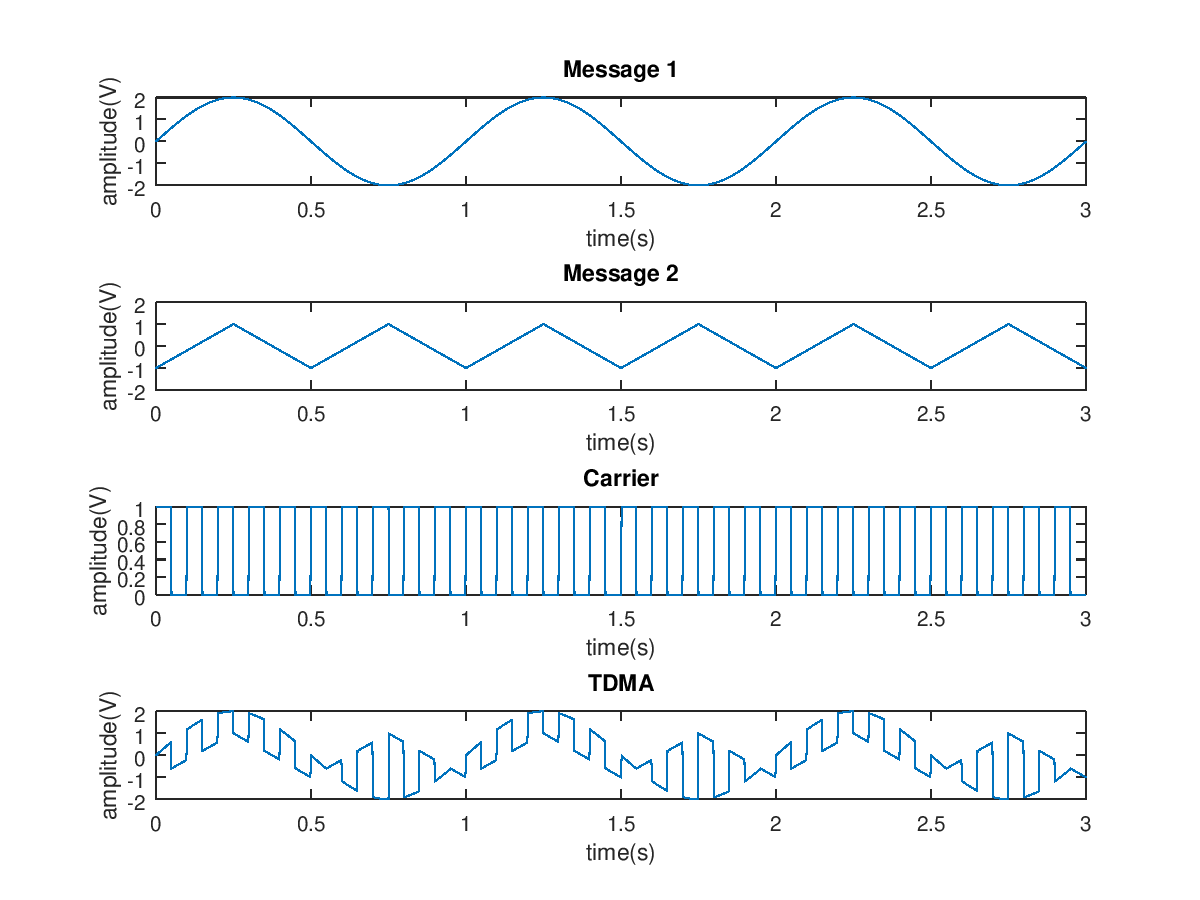
\includegraphics[width=0.8\textwidth]{tdmawaves.png}
	\caption{Time Division Multiple Access: sample waveforms}
	\label{tdmawaveforms}
\end{figure}


\section*{Design}

A sinusoidal signal and a triangular signal  will serve as the two signals to be multiplexed. A binary  valued control signal controls the time over which for switching IC circuits. The binary sequence switches the sinusoidal signal to output during its ON period and the inverted binary sequence switches the triangular signal to output during its OFF period. The two outputs are combined at the load resistor $R_L =1 k\Omega$. See Figure \ref{tdma} for modulation circuit.


\section*{Circuit Diagram}

The TDMA circuit using analog switching IC 4046 is shown in Figure \ref{tdma}.

\begin{figure}[h]
	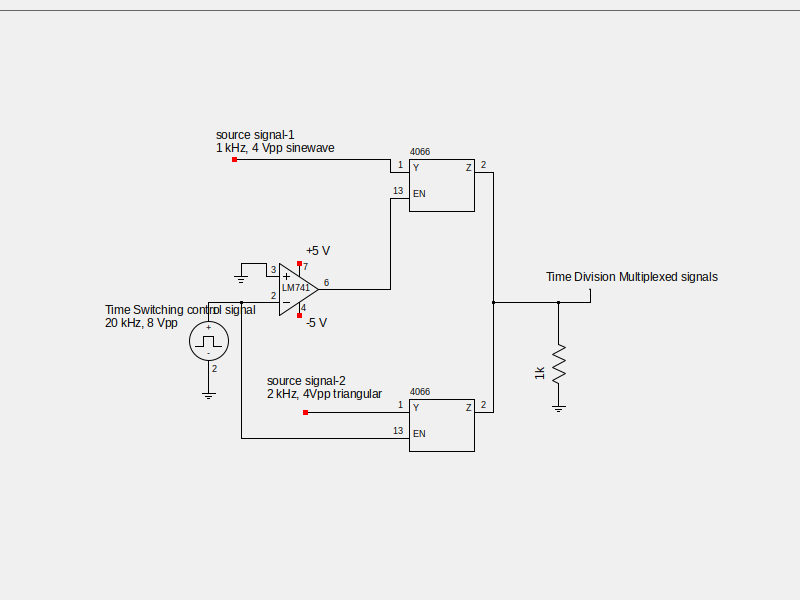
\includegraphics[width=0.8\textwidth]{tdma.png}
	\caption{TDMA Modulator}
	\label{tdma}
\end{figure}

\clearpage
\section*{Procedure}
\begin{itemize}
\item
Connect the TDMA generating circuit as shown in the circuit diagram, Figure \ref{tdma}.
\item
Feed the carrier signal-1 ($4 V_{pp}, 1 kHz$ sine wave) and the carrier signal-2 $4 V_{pp}, 2 kHz$ triangular wave) from the function generator.
\item
Feed the control signal  ($8 V_{pp}, 20 kHz$ square wave) from another function generator.
\item
Observe the output on a CRO and plot the graphs of the input and output waveforms.

\end{itemize}
\section*{Observation}
Plot the graphs of input and output waveforms as observed on a CRO.
\section*{Result}

Implemented the Time division multiplexing circuit and observed the output waveforms.
